% \label{Results}

This chapter finally brings together both the Hidden Markov only Model and the Generalised HMM for rainfall. We begin with discussing what data we have available before a graphical comparison of Cumulative Distribution Functions (CDFs) and analysing numerically using the Kolmogorov–Smirnov test \ref{Model_Selection:Kolmogorov_Smirnov_Test}.

\section{Datasets}
\label{Results:Datasets}
Before we begin testing, we summarise what data we have so far. 

Each month has 2138 days of rainfall data. Due to unforeseen issues with the Baum-Welch algorithm, we used only 1000 of this for training. The remaining 1138 have been left aside for out-of-sample testing. If our simulations fit this dataset, it is a strong indication of success, as fitting the training set could mean the model has fit the given data and not the generalised case. Thus we have two sets of recorded data; the training of size 1000 and the test of size 1138.

When we first created our HMM in \ref{Simple_Rainfall_HMM} we also generated a simulation of size 1000 days. We will use this simulation for our testing now. From our parameter estimates in \ref{Generalising_the_Observation_Matrix:Parameter_Estimation} we generated simulations of size 1000 using "generator", which can be found in the "Model Generator" folder. 

Therefore we now have four data sets, two recorded, training and test,  and two simulated, HMM only and our Generalised HMM model.


\section{Analysis}
\label{Results:Analysis}

In this section, we finally analyse both our simulations both graphically and numerically to help decide whether HMMs provide any use to rainfall modelling.

    \subsection{CDFs}
    \label{Results:Analysis:CDFs}
    We begin by comparing the empirical cumulative distribution functions of the observed data and both simulations. For the recorded data, we combine the training and test data.

    \begin{figure}
        \begin{subfigure}{.3\textwidth}
          \centering
          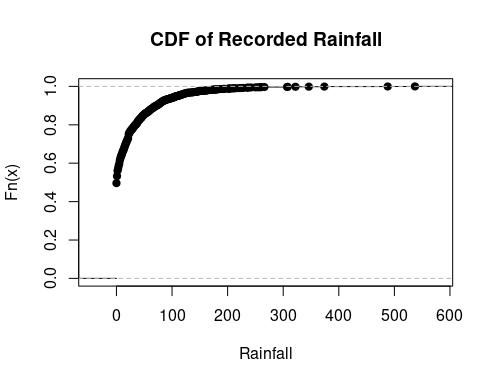
\includegraphics[width=\linewidth]{CDF/recorded.png}
          \caption{}
          \label{CDF:data}
        \end{subfigure}
        \begin{subfigure}{.3\textwidth}
          \centering
          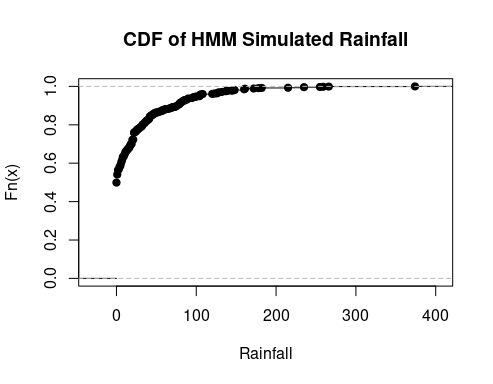
\includegraphics[width=\linewidth]{CDF/HMM.png}
          \caption{}
          \label{CDF:simhmm}
        \end{subfigure}
        \begin{subfigure}{.3\textwidth}
          \centering
          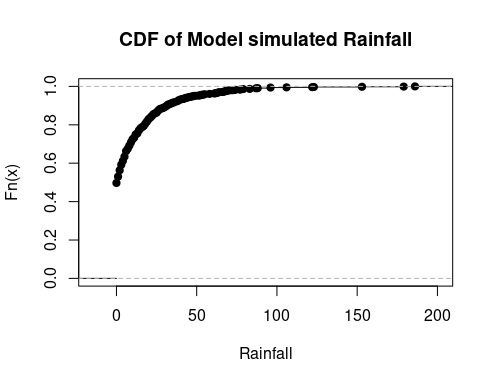
\includegraphics[width=\linewidth]{CDF/model.png}
          \caption{}
          \label{CDF:model}
        \end{subfigure}
        \caption{}
        \label{CDF}
    \end{figure}
    
    From Figure~\ref{CDF} we can instantly see that neither the HMM only nor our generalised model simulates any extreme values observed in the recorded data. However, the shape of the graphs does seem similar. It is also clear that the rate increases much faster for both recorded and HMM only datasets. This result suggests our generalised model may not be a good fit.


    \subsection{Kolmogorov–Smirnov tests}
    \label{Results:Analysis:Kolmogorov_Smirnov_tests}

    To obtain numerical results, we apply the Kologmorov-Smirnoff (KS) test for two samples \ref{Model_Selection:Kolmogorov_Smirnov_Test}. We apply this to both of our models against both training and test data. Our hypotheses are given as follows:

    \begin{itemize}
        \item $H_0$: The two samples are from the same distribution
        \item $H_1$: The two samples are not from the same distribution.
    \end{itemize}

    We will use a 5\% significance level for testing. Thus if the p-value is smaller than 0.05, we will reject the null hypothesis. We record all four p-values for each month in the table given below.

    \begin{center}
        \begin{tabular}{c | c | c | c | c}
                &  Train & Train     & Test &  Test \\  
                \hline
            Month & HMM    & Gen Model & HMM  &  Gen Model\\
            \hline
            0     &   0.8593  &   \num{4.939e-5}     &   0.7899          &       \num{4.60e-08}   \\
            1     &   0.9969  &   0.002038          &   0.105           &        \num{5.46e-06}   \\
            2     &   1       &   \num{2.13e-05}     &   0.1118          &       \num{7.65e-07}   \\
            3     &   1       &   \num{1.79e-06}     &   0.02163         &       \num{1.11e-07}   \\
            4     &   0.4324  &   \num{1.38e-05}     &   0.0009582       &       \num{7.98e-08}   \\
            5     &   1       &   0.006202          &   0.2979          &       0.0004948  \\
            6     &   1       &   \num{1.11e-05}     &   0.1809          &       \num{8.53e-08}   \\
            7     &   1       &   \num{2.13e-05}     &   0.03555         &       \num{4.53e-05}   \\
            8     &   0.9999  &   0.0001108         &   0.07192         &       0.001033   \\
            9     &   0.9969  &   \num{6.06e-05}     &   \num{5.22e-07}   &       \num{1.22e-07}   \\
            10    &   0.8879  &   0.0008667         &   0.1914          &       \num{9.07e-05}   \\
            11    &   0.9999  &   \num{6.06e-05}     &   0.265           &       \num{2.15e-06}  

        \end{tabular}
    \end{center}


    It is clear to see that for all months, the KS test produces non-rejections. Thus one can assume the HMM describes the training data. For the test data, we can see that we rejected the null hypothesis for 4 out of 12 months. To justify this result, we require further testing. Initial thoughts include: maybe the training data was more similar to the test for the 8 that did not reject, or maybe the optima found through Baum-welch was not, in fact, a suitable optimum. 

    For our generalised model, we rejected the null hypothesis whenever tested against both training and test sets. This result suggests the model is not describing the rainfall data well. 